% $Id: template.tex 11 2007-04-03 22:25:53Z jpeltier $

\documentclass{vgtc}                          % final (conference style)
%\documentclass[review]{vgtc}                 % review
%\documentclass[widereview]{vgtc}             % wide-spaced review
%\documentclass[preprint]{vgtc}               % preprint
%\documentclass[electronic]{vgtc}             % electronic version

%% Uncomment one of the lines above depending on where your paper is
%% in the conference process. ``review'' and ``widereview'' are for review
%% submission, ``preprint'' is for pre-publication, and the final version
%% doesn't use a specific qualifier. Further, ``electronic'' includes
%% hyperreferences for more convenient online viewing.

%% Please use one of the ``review'' options in combination with the
%% assigned online id (see below) ONLY if your paper uses a double blind
%% review process. Some conferences, like IEEE Vis and InfoVis, have NOT
%% in the past.

%% Figures should be in CMYK or Grey scale format, otherwise, colour
%% shifting may occur during the printing process.

%% These few lines make a distinction between latex and pdflatex calls and they
%% bring in essential packages for graphics and font handling.
%% Note that due to the \DeclareGraphicsExtensions{} call it is no longer necessary
%% to provide the the path and extension of a graphics file:
%% \includegraphics{diamondrule} is completely sufficient.
%%
\ifpdf%                                % if we use pdflatex
	\pdfoutput=1\relax                   % create PDFs from pdfLaTeX
	\pdfcompresslevel=9                  % PDF Compression
	\pdfoptionpdfminorversion=7          % create PDF 1.7
	\ExecuteOptions{pdftex}
	\usepackage{graphicx}                % allow us to embed graphics files
	\DeclareGraphicsExtensions{.pdf,.png,.jpg,.jpeg} % for pdflatex we expect .pdf, .png, or .jpg files
\else%                                 % else we use pure latex
	\ExecuteOptions{dvips}
	\usepackage{graphicx}                % allow us to embed graphics files
	\DeclareGraphicsExtensions{.eps}     % for pure latex we expect eps files
\fi%

%% it is recomended to use ``\autoref{sec:bla}'' instead of ``Fig.~\ref{sec:bla}''
\graphicspath{{figures/}{pictures/}{images/}{./}} % where to search for the images

\usepackage{microtype}                 % use micro-typography (slightly more compact, better to read)
\PassOptionsToPackage{warn}{textcomp}  % to address font issues with \textrightarrow
\usepackage{textcomp}                  % use better special symbols
\usepackage{mathptmx}                  % use matching math font
\usepackage{times}                     % we use Times as the main font
\renewcommand*\ttdefault{txtt}         % a nicer typewriter font
% \usepackage{cite}                      % needed to automatically sort the references
\usepackage{tabu}                      % only used for the table example
\usepackage{booktabs}                  % only used for the table example
%% We encourage the use of mathptmx for consistent usage of times font
%% throughout the proceedings. However, if you encounter conflicts
%% with other math-related packages, you may want to disable it.


%% If you are submitting a paper to a conference for review with a double
%% blind reviewing process, please replace the value ``0'' below with your
%% OnlineID. Otherwise, you may safely leave it at ``0''.
\onlineid{0}

%% declare the category of your paper, only shown in review mode
\vgtccategory{Research}

%% allow for this line if you want the electronic option to work properly
\vgtcinsertpkg

%% In preprint mode you may define your own headline. If not, the default IEEE copyright message will appear in preprint mode.
%\preprinttext{To appear in an IEEE VGTC sponsored conference.}

%% This adds a link to the version of the paper on IEEEXplore
%% Uncomment this line when you produce a preprint version of the article
%% after the article receives a DOI for the paper from IEEE
%\ieeedoi{xx.xxxx/TVCG.201x.xxxxxxx}


%% Paper title.

\title{VisCPU: visualizing performance of stream processing applications executed on CPU}

%% This is how authors are specified in the conference style

%% Author and Affiliation (single author).
%%\author{Roy G. Biv\thanks{e-mail: roy.g.biv@aol.com}}
%%\affiliation{\scriptsize Allied Widgets Research}

%% Author and Affiliation (multiple authors with single affiliations).
\author{
	Claudio Scheer\thanks{e-mail: claudio.scheer@edu.pucrs.br} %
	\and Dalvan Griebler\thanks{e-mail: dalvan.griebler@edu.pucrs.br} %
	\and Isabel Harb Manssour\thanks{e-mail: isabel.manssour@pucrs.br}
}
\affiliation{\scriptsize Pontifical Catholic University of Rio Grande do Sul - PUCRS \\ Brazil}

%% Author and Affiliation (multiple authors with multiple affiliations)
% \author{
%     Claudio Scheer\thanks{e-mail: claudio.scheer@edu.pucrs.br}\\ %
% 	% \scriptsize Starbucks Research %
% 	\and Isabel Harb Manssour\thanks{e-mail: isabel.manssour@pucrs.br}\\ %
% 	% \scriptsize Grimley Widgets, Inc. %
% 	\and Dalvan Griebler\thanks{e-mail: dalvan.griebler@edu.pucrs.br}\\ %
% 	% \parbox{1.4in}{\scriptsize \centering Martha Stewart Enterprises \\ Microsoft Research}
% }

%% A teaser figure can be included as follows, but is not recommended since
%% the space is now taken up by a full width abstract.
%\teaser{
%  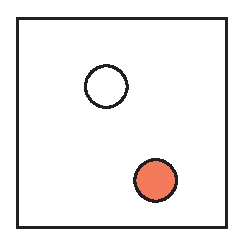
\includegraphics[width=1.5in]{sample.eps}
%  \caption{Lookit! Lookit!}
%}

%% Abstract section.
\abstract{
	Tracking performance metrics of applications is indispensable to identify bottlenecks or even where resources should be applied to fix performance issues. Perf is a tool that captures performance metrics from the hardware where the application was executed. However, data captured by Perf can be hard to read and, in some cases, impossible due to the large size of the generated files. Therefore, we propose in this paper a visualization dashboard for data captures using Perf: VisPerf. VisPerf implements a data pipeline from capturing to visualizing data. The dashboard allows the user to compare specific experiments and to see how hardware events varied between these experiments. VisPerf is still in the prototype phase. Therefore, requires some validations, especially with application developers who may take benefits from VisPerf.

} % end of abstract

%% ACM Computing Classification System (CCS).
%% See <http://www.acm.org/about/class> for details.
%% We recommend the 2012 system <http://www.acm.org/about/class/class/2012>
%% For the 2012 system use the ``\CCScatTwelve'' which command takes four arguments.
%% The 1998 system <http://www.acm.org/about/class/class/2012> is still possible
%% For the 1998 system use the ``\CCScat'' which command takes four arguments.
%% In both cases the last two arguments (1998) or last three (2012) can be empty.

\CCScatlist{
	\CCScatTwelve{Human-centered computing}{Visu\-al\-iza\-tion}{Visu\-al\-iza\-tion techniques}{Treemaps};
	\CCScatTwelve{Human-centered computing}{Visu\-al\-iza\-tion}{Visualization design and evaluation methods}{}
}

%\CCScatlist{
%\CCScat{H.5.2}{User Interfaces}{User Interfaces}{Graphical user interfaces (GUI)}{};
%\CCScat{H.5.m}{Information Interfaces and Presentation}{Miscellaneous}{}{}
%}

%% Copyright space is enabled by default as required by guidelines.
%% It is disabled by the 'review' option or via the following command:
% \nocopyrightspace

%%%%%%%%%%%%%%%%%%%%%%%%%%%%%%%%%%%%%%%%%%%%%%%%%%%%%%%%%%%%%%%%
%%%%%%%%%%%%%%%%%%%%%% START OF THE PAPER %%%%%%%%%%%%%%%%%%%%%%
%%%%%%%%%%%%%%%%%%%%%%%%%%%%%%%%%%%%%%%%%%%%%%%%%%%%%%%%%%%%%%%%%

\begin{document}

%% The ``\maketitle'' command must be the first command after the
%% ``\begin{document}'' command. It prepares and prints the title block.

%% the only exception to this rule is the \firstsection command
\firstsection{Introduction}

\maketitle

%% \section{Introduction} %for journal use above \firstsection{..} instead
This is the introduction.


\section{Related Works}

In this section, we discuss papers that proposed visualization techniques to better understand data captured by Perf.

We selected papers related to visualization of Perf data
Discuss the related works.

\begin{itemize}
	\item https://dl.acm.org/doi/10.1145/2909476: The flame graph
\end{itemize}

\section{Perf}

Perf is a profiling tool included in the Linux kernel. It can be used to capture CPU performance counters, tracepoints, kprobes\footnote{\url{https://www.kernel.org/doc/html/latest/trace/kprobes.html}}, and uprobes\footnote{\url{https://www.kernel.org/doc/html/latest/trace/uprobetracer.html}}~\cite{perf_wiki}. Perf also supports software events, such as page misses. In turn, tracepoints are placed in the source code to collect timestamps and stack traces and performance counters are hardware registers that count events of the CPU, such as instructions executed and cache-misses. Perf has low overhead, as it is integrated into the kernel. Moreover, Perf supports counters in different architectures. Therefore, it can be used to profile applications in different Intel architectures or even in AMD CPUs.

There are several subcommands available in Perf. Below we describe some of the subcommands:

\begin{itemize}
	\item \texttt{perf stat}: gather performance counter statistics from a command;
    \item \texttt{perf record}: run a command and record its profile for later analysis. By default, profile is saved in a file named \texttt{perf.data};
    \item \texttt{perf report}: read \texttt{perf.data} and display the profile recorded in this file;
    \item \texttt{perf script}: read \texttt{perf.data} and display the trace recorded in this file;
	\item \texttt{perf top}: display performance counter profile in real time;
	\item \texttt{perf list}: list events available to be captured in the current architecture;
\end{itemize}

\texttt{perf list} shows events from several sources, such as hardware and software. Hardware events are provided by the processor and its PMUs (Performance Monitoring Unit), which may vary among different companies. Next, we discuss the counters captured in our experiments~\cite{intel_pmu}.

\begin{itemize}
	\item \textbf{cpu-cycles}: number of fetch-decode-execute cycles the CPU executed;
	\item \textbf{instructions}: number of instructions the CPU executed;
	\item \textbf{cache-misses}: number of cache-misses;
	\item \textbf{cache-references}: number of references found in cache;
	\item \textbf{L1-dcache-load-misses}: number of misses when loading data from L1 cache;
	\item \textbf{L1-dcache-loads}: number of data loads from L1 cache;
	\item \textbf{L1-dcache-stores}: number of data stores made in L1 cache;
	\item \textbf{L1-icache-load-misses}: number of misses when loading instructions from L1 cache;
	\item \textbf{L1-icache-loads}: number of instructions load from L1 cache;
	\item \textbf{L1-icache-stores}: number of instructions store made in L1 cache;
	\item \textbf{LLC-loads}: number of references loaded from LLC (Last Level Cache, usually L3);
	\item \textbf{LLC-load-misses}: number of references missed when loading from LLC;
	\item \textbf{LLC-stores}: number of references store made loading in LLC;
	\item \textbf{mem-stores}: number of stores made in the main memory;
	\item \textbf{mem-loads}: number of loads made from the main memory;
	\item \textbf{branch-misses}: number of mispredicted speculative branches;
    \item \textbf{branch-instructions}: number of correct speculative branches;
	\item \textbf{bus-cycles}: number of CPU cycles needed to fetch or write data to the main memory, for example;
\end{itemize}

For this paper, we profiled the person recognition application. The main goal of this application is to recognize is there is a person in a specific image, using OpenCV. To characterize a stream processing application, it is, we cannot predict when data will stop entering the application, we used a video as input.

Towards exploiting parallelism, we use the FastFlow library and compared two mapping policies. In summary, the mapping policy defines in which core threads launched by the application will be placed. We profiled the person recognition application using the default mapping policy os the Linux operating system and the mapping policy proposed by FastFlow.

\section{VisCPU}

\subsection{Data Pre-processing}

Explain what we did.

\section{Conclusion}


%% if specified like this the section will be committed in review mode
\acknowledgments{Thanks!
}

%\bibliographystyle{abbrv}
\bibliographystyle{abbrv-doi}
%\bibliographystyle{abbrv-doi-narrow}
%\bibliographystyle{abbrv-doi-hyperref}
%\bibliographystyle{abbrv-doi-hyperref-narrow}

\bibliography{references}
\end{document}
